\chapter{Resultados e Discussão}
\label{chap:resultados}

Neste capítulo, são abordados, analisados e discutidos os resultados encontrados
durante a exploração do tema e das plataformas e durante a implementação das
aplicações, além de verificar a precisão atingida com a aplicação implementada.


\section{Método de teste}
\label{sec:metodo-teste}

Como discutido no \autoref{chap:Construcao}, a arquitetura geral da aplicação (\autoref{fig-arq-app})
mostra que a precisão vista na aplicação \emph{Web} depende dos resultados
encontrados pela aplicação sensor que, por sua vez, depende do par de
capacidades combinadas do \emph{hardware} adaptador Wi-Fi e do \emph{software}
\emph{TShark}. Portanto, a metodologia de testes empregada neste capítulo é
analisar diretamente as capacidades deste último par. Esta decisão também se
deve pela facilidade de armazenar e analisar arquivos CSV gerados pelo
\emph{TShark}.

As capturas foram executadas com o comando descrito no \autoref{code-tshark-pipe-assinc}
que é o mesmo utilizado na aplicação sensor.

\begin{lstlisting}[language=bash,caption={TShark e redirecionamento da saída para arquivo assíncrono},label=code-tshark-pipe-assinc]
pi@sensor-01:~ $ tshark -I -i wlan0 -T fields -E header=y -E quote=d \
-e wlan.sa -e wlan.sa_resolved -e wlan.ta -e wlan.ta_resolved \
-e radiotap.dbm_antsignal -e wlan_mgt.ssid \
>> 2017-01-17--02-48--rpi-02.csv &
pi@sensor-01:~ $ exit
\end{lstlisting}

Neste modo de uso, os resultados são direcionadas para a saída padrão
(stdout)  do terminal e podem ser capturados por outro programa no formato
de valores separados por vírgula (CSV). Os campos escolhidos para captura
são \emph{wlan.sa}, \emph{wlan.sa\_resolved}, \emph{wlan.ta},
\emph{wlan.ta\_resolved}, \emph{radiotap.dbm\_antsignal} e \emph{wlan\_mgt.ssid}.

Na linha 4 do \autoref{code-tshark-pipe-assinc}, o \emph{\&} representa o início
de um processo independente (assíncrono) e, a linha 5, a finalização do terminal.
Esta operação foi somente executada durante a captura longa.

A análise de dados foi feita com a função \emph{summary} da ferramenta
\emph{Ron’s editor}\footnote{\url{https://www.ronsplace.eu/Products/RonsEditor}}
e a filtragem com a função \emph{Filter} da ferramenta
\emph{RecCsvEditor}\footnote{\url{http://recsveditor.sourceforge.net/}}. Para a
construção dos gráficos, foi utilizada a ferramenta
\emph{WPS Spreadsheets}\footnote{\url{https://www.wps.com/office-free}}.

\clearpage
\section{Avaliação de ruído e consistência}
\label{sec:teste-ruido}


Para entender o ambiente onde a aplicação foi desenvolvida e testada no âmbito
de ruído e pontos de referência Wi-Fi foi executada uma captura de referência
durante a noite quando ninguém habitava o prédio prototipo portanto nenhum
dispositivo foi movimentado até a manhã seguinte.

Nesta captura dois sensores foram utilizados posicionados a menos de 10
centímetros de distância um do outro sobre uma mesa a um metro do chão no ponto
azul de legenda \emph{'sensor 2'} idicado na \autoref{fig-planta-baixa}. A captura
ocorreu de \emph{2:50} até aproximadamente \emph{11:25} totalizando aproximadamente 8 horas de
captura.

\begin{figure}[htb]
	\caption{\label{fig-planta-baixa}Ambiente de teste}
	\begin{center}
		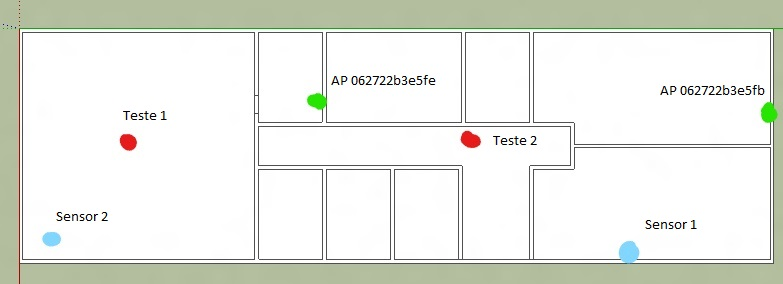
\includegraphics[width=1\textwidth]{060-testes/data-analisis/planta-baixa_Ink_LI.jpg}
	\end{center}
	\legend{Fonte: Elaborada pelo autor}
	\nota[Em azul]{Sensores da aplicação}%
	\nota[Em verde]{Pontos de acesso da rede Wi-Fi do laboratório}%
	\nota[Em verbelho]{Pontos do dispositivo teste}%
\end{figure}


Para o primeiro sensor o sumário indicou que foram capturados \emph{1 729 624}
pacotes num arquivo de \emph{155 MB} com \emph{88} transmissores únicos.
Para o segundo sensor o sumário indicou que foram capturados \emph{1 554 319}
pacotes num arquivo de \emph{134 MB} com \emph{66} transmissores únicos.
Em ambos os sensores se destacaram dois endereços MAC que são os pontos de
acesso para rede Wi-Fi do laboratório.

Os pacotes capturados dos pontos de acesso e os valores de potência de sinal
associados são notáveis para entender a precisão de um sistema de localização
desta categoria uma vez que os pontos de acesso estão fixos e trasmitiram o
maior número de pacotes nesta captura.

Nas \autoref{fig-062722b3e5fb-s1}, \autoref{fig-062722b3e5fb-s2},
\autoref{fig-062722b3e5fe-s1} e \autoref{fig-062722b3e5fe-s2} podemos observar
a potência de sinal para cada pacote capturado em ordem de chegada.

\begin{figure}[htb]
	\begin{minipage}{0.49\textwidth}
	\centering
		\caption{\label{fig-062722b3e5fb-s1}Sinal em dBm por pacote capturado - 062722b3e5fb sensor 1}
		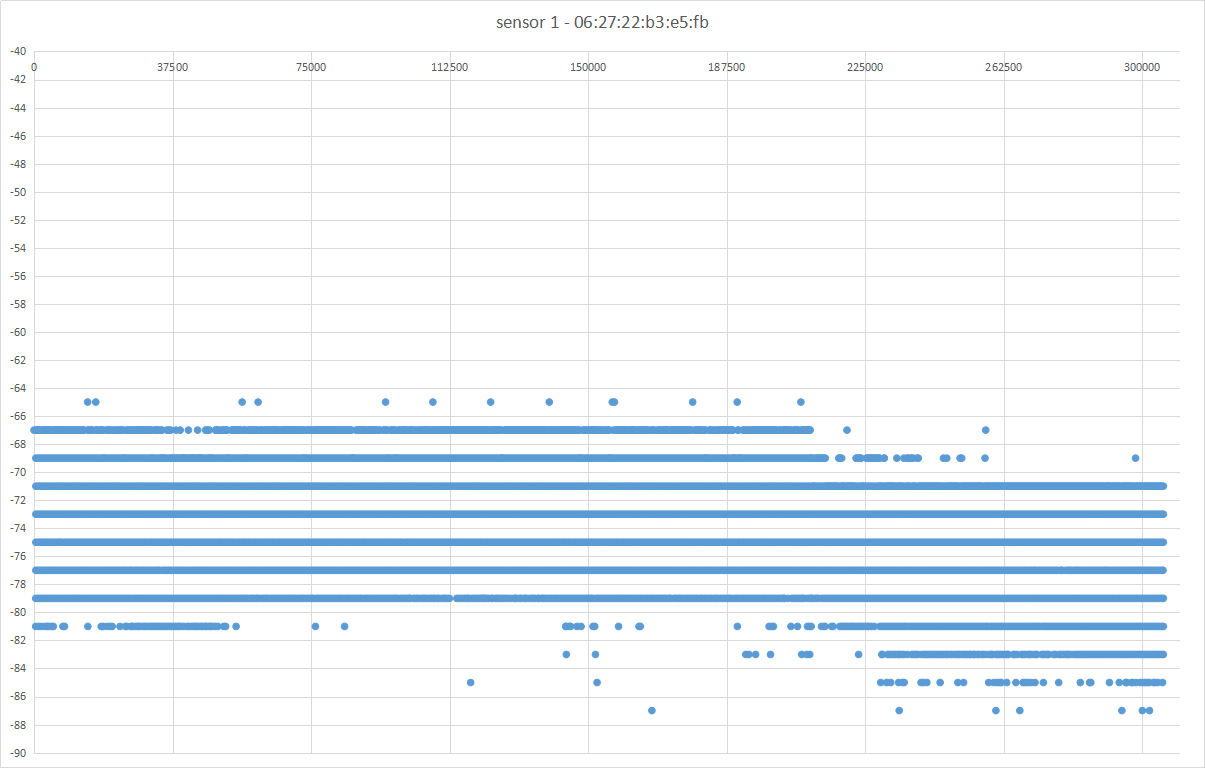
\includegraphics[width=1\textwidth]{060-testes/data-analisis/night-run/062722b3e5fb-sensor-01.png}
		\legend{Fonte: Elaborada pelo autor}
	\end{minipage}
\hfill
	\begin{minipage}{0.49\textwidth}
	\centering
		\caption{\label{fig-062722b3e5fb-s2}Sinal em dBm por pacote capturado - 062722b3e5fb sensor 2}
		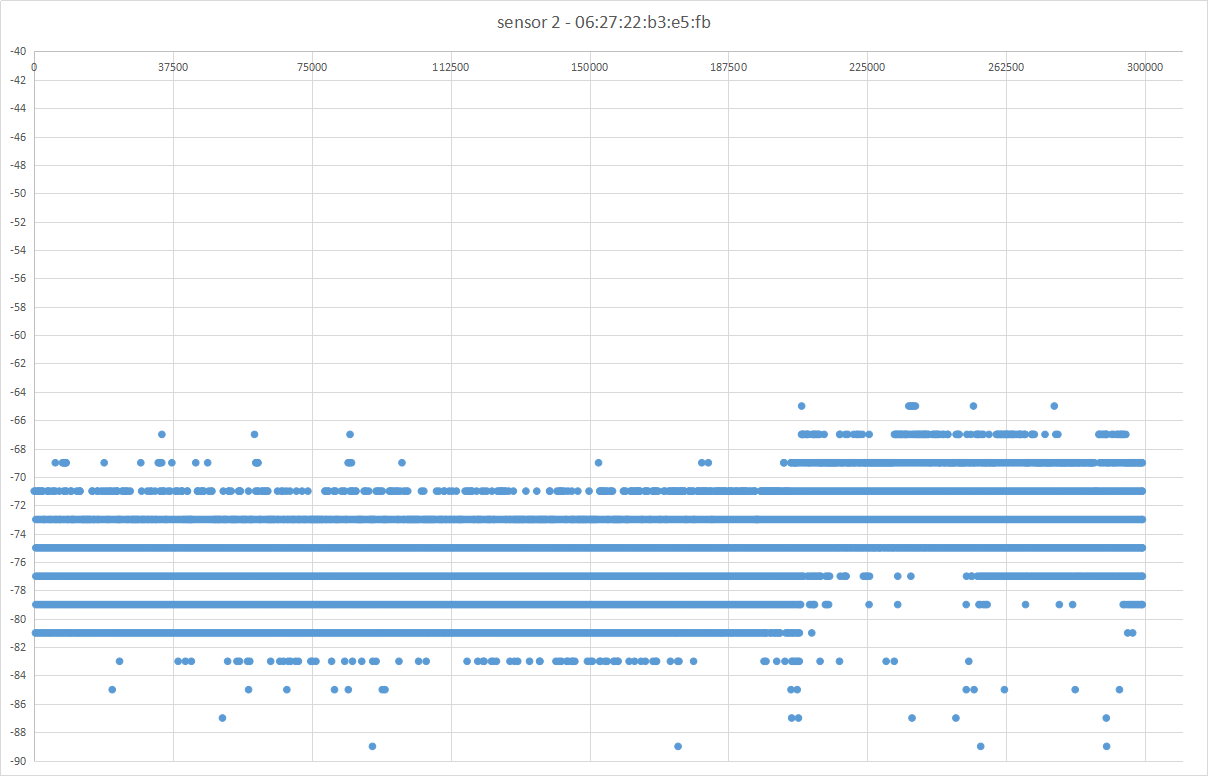
\includegraphics[width=1\textwidth]{060-testes/data-analisis/night-run/062722b3e5fb-sensor-02.png}
		\legend{Fonte: Elaborada pelo autor}
	\end{minipage}
\hfill
	\begin{minipage}{0.49\textwidth}
	\centering
		\caption{\label{fig-062722b3e5fe-s1}Sinal em dBm por pacote capturado - 062722b3e5fe sensor 1}
		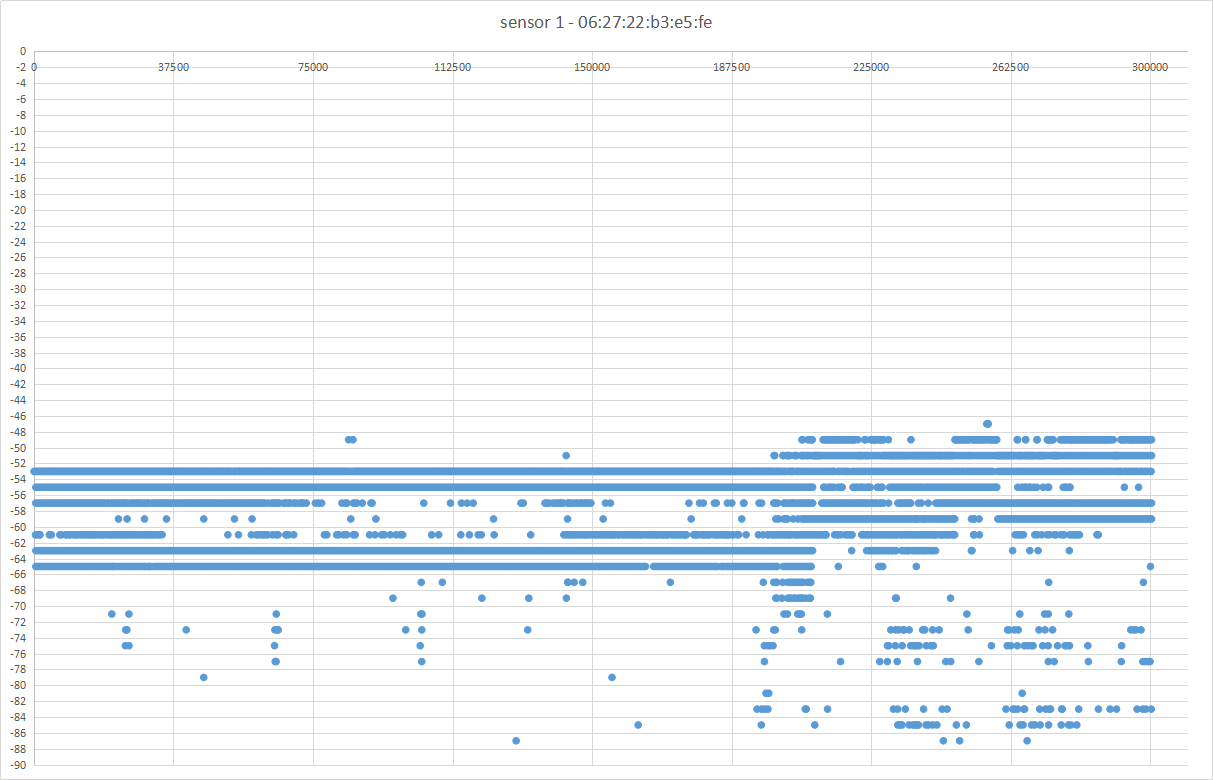
\includegraphics[width=1\textwidth]{060-testes/data-analisis/night-run/062722b3e5fe-sensor-01.png}
		\legend{Fonte: Elaborada pelo autor}
	\end{minipage}
\hfill
	\begin{minipage}{0.49\textwidth}
	\centering
		\caption{\label{fig-062722b3e5fe-s2}Sinal em dBm por pacote capturado - 062722b3e5fe sensor 2}
		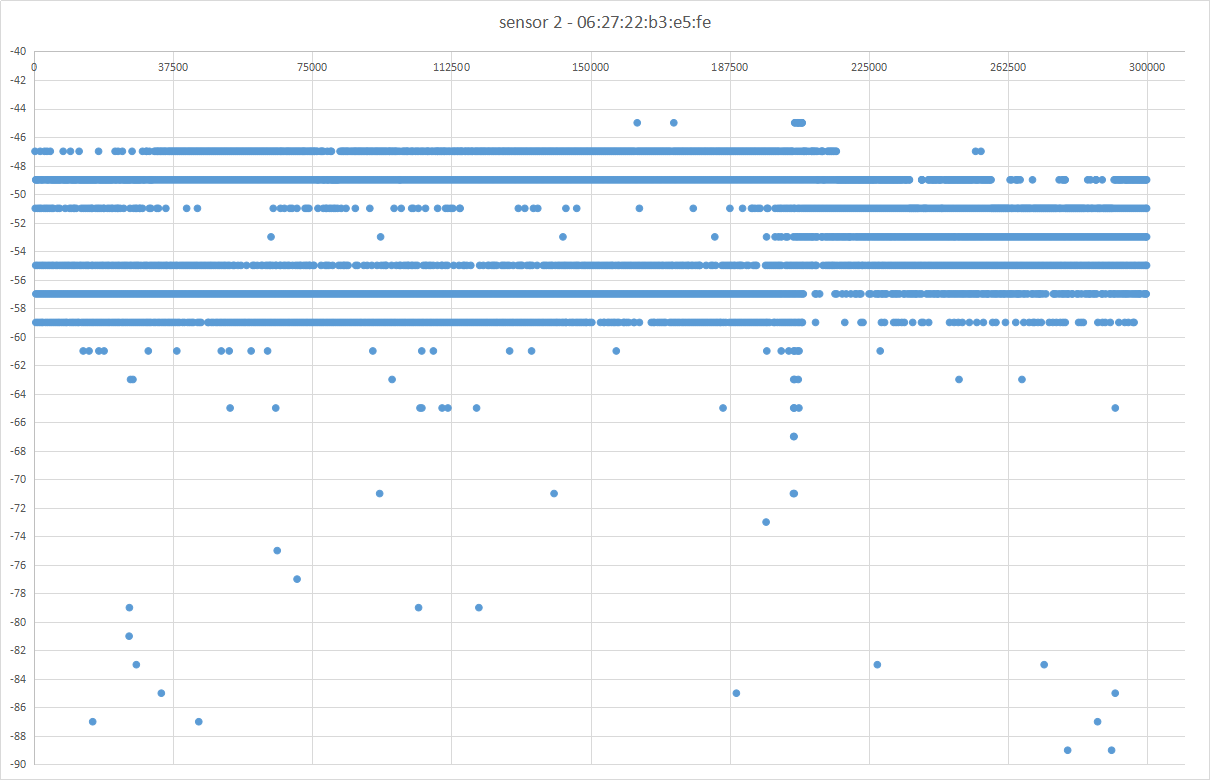
\includegraphics[width=1\textwidth]{060-testes/data-analisis/night-run/062722b3e5fe-sensor-02.png}
		\legend{Fonte: Elaborada pelo autor}
	\end{minipage}
\end{figure}

Imediatamente percebe-se que, apesar da distância ser invariável durate todo o
teste, ela não permaneceu remotamente constante. Nota-se também que o valor
nunca assume valor par. Estas duas características fazem com que o gráfico
seja feito de 7 linhas paralelas ao centro e alguns grupos de pontos ao redor.

Nota-se também uma abrupta mudança no comportamento próximo do pacote 225 000.
Estimou-se que esta mudança é devido ao horário (08:00) em que a universidade
(incluindo o prédio piloto e seus arredores) inicia o seu funcionamento.

Para ter uma visão geral clara da distribuição das potências de sinal calculamos
a média e o desvio padrão para cada um dos casos. Além disso adicionamos o
quanto o desvio padrão representa da média (erro).

\begin{table}[htb]
\IBGEtab{%
\ABNTEXchapterfont {
	\caption{\label{table:ap-pwr-avg}dBm Pontos de acesso - Acumulado 8 horas}%
}
}{%
\begin{tabular}{c|cc|cc}
\toprule
\midrule
AP							& \multicolumn{2}{c}{06:27:22:b3:e5:fe}		&	\multicolumn{2}{c}{06:27:22:b3:e5:fb}	\\
							&	Sensor 1		&	Sensor 2			&	Sensor 1		&	Sensor 2			\\
\midrule
Pacotes						&	300403			&	299864				&	305735			&	299264				\\
\midrule
Média						& 	-57.66137822	&	-52.57644132		&	-73.04459417	&	-76.12900984		\\
\midrule
$\sigma$ (Desvio Padrão)	&	4.746974756		&	3.712407998			&	3.05045545		&	2.889560991			\\
$\sigma$ \%					&	8\%				&	7\%					&	4\%				&	4\%					\\
\midrule
%$3 \times \sigma $			&	14.24092427		&	11.13722399			&	9.151366351		&	8.668682972			\\
%$3 \times \sigma $ \%		&	25\%			&	21\%				&	13\%			&	11\%				\\
%\midrule
\bottomrule
\end{tabular}%
}{%
	\fonte{Produzido pelo autor.}%
}
\end{table}


Em alguns trabalhos podemos
encontrar a equação de FSPL (\emph{Free-space path loss} - perca no caminho em
espaço aberto) que é usualmente utilizada para determinar a potência do sinal
a ser transmitido para que este alcance o seu destinatário.

\begin{equation}
	{\mbox{FSPL(dB)}}=20\log _{{10}}(\text{distância})+20\log _{{10}}(\text{frequência})+92.45
\end{equation}

Na aplicação \emph{Android} \emph{Wifi Distance Calculator} \cite{Kuik2016} e
http://rvmiller.com/2013/05/part-1-wifi-based-trilateration-on-android/
a seguinte equação é utilizada.

\begin{equation}
	\text{distância} = 10 ^{ \frac{ \text{potência do sinal} - 20 \times log_{10}\left(\text{frequência}\right)  + 27.55}{20} }
\end{equation}



Além disso, a definição do padrão IEEE 802.11 inclui que a potência de sinal
utilizada por uma estação para transmissão pode ser variada e a implementação
do método escolhido para a escolha da potência não faz parte do padrão.

\begin{citacao}[english]

	A STA may use any criteria, and in particular any path loss and link margin
	estimates, to dynamically adapt the transmit power for transmissions of an
	MPDU to another STA. The adaptation methods or criteria are beyond the scope
	of this standard. \

	\citeonline[10.8.6,p. 1047]{ieee80211}
\end{citacao}

Portanto


\clearpage
\section{Teste relação de distância com smartphone como objetivo}
\label{sec:teste-smarphone}

Para verificar a capacidade do sensores de localizar contextualmente um
dispositivo móvel, smartphone, foi utilizado. Este foi posicionado em duas salas
diferentes, em cada uma das salas foi executada uma captura de 10 minutos. Para
que houvesse tráfego na rede o dispositivo móvel foi configurado para receber um
stream de vídeo no aplicativo \emph{Netflix}.

A captura foi realizada utilizando a ferramenta TShark da mesma maneira que é utilizada no
aplicativo. A descrição deste modo de operação pode ser encontrada no capítulo de construção.

\begin{lstlisting}[language=bash,caption={TShark e redirecionamento da saída para arquivo},label=code-tshark-pipe]
pi@sensor-01:~ $ tshark -I -i wlan1 -T fields -E separator=, -E quote=d \
-e wlan.sa -e wlan.sa_resolved -e wlan.ta -e wlan.ta_resolved \
-e radiotap.dbm_antsignal -e wlan_mgt.ssid >> sensor-02-distance-test-01.csv
pi@sensor-01:~ $
\end{lstlisting}

Para o primeiro caso o dispositivo estava na mesma sala do sensor número 2 que é a maior
sala do prédio com 12  metros de comprimento por 10 metros  De largura. neste caso foram
capturados 157736 pacotes totalizando 9.7 megabytes pelo sensor 1 21974 pacotes totalizando
1.9 megabytes de captura pelo sensor 2.

No segundo teste o dispositivo móvel estava posicionado no corredor fora da sala do sensor 1
e distante do sensor 2.  neste teste o sensor 1 capturou 103555 pacotes totalizando 6.4 megabytes
de captura e o sensor 2 capturou 22635 pacotes totalizando 2 megabytes de captura

Posteriormente os arquivos de captura foram analisados com a ferramenta
\emph{Ron’s Editor} para que um sumário fosse construído.

\begin{figure}[htb]
	\label{mg4-noise}
	\centering
	\begin{minipage}{0.49\textwidth}
	\centering
		\caption{\label{fig-mg4-noise-t1}Captura total (noise) - Teste 1}
		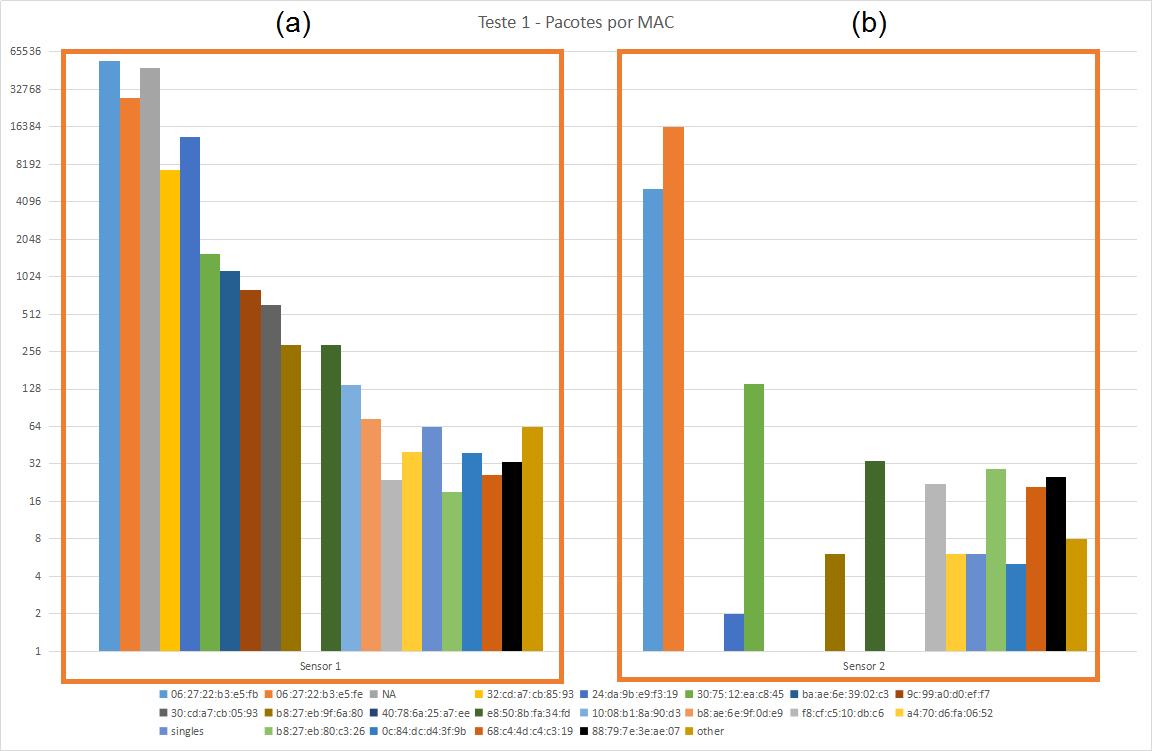
\includegraphics[width=1\textwidth]{060-testes/data-analisis/distance-mg4plus-netflix/Teste1.png}
		\legend{Fonte: Elaborada pelo autor}
	\end{minipage}
	\hfill
	\begin{minipage}{0.49\textwidth}
	\centering
		\caption{\label{fig-mg4-noise-t2}Captura total (noise) - Teste 2}
		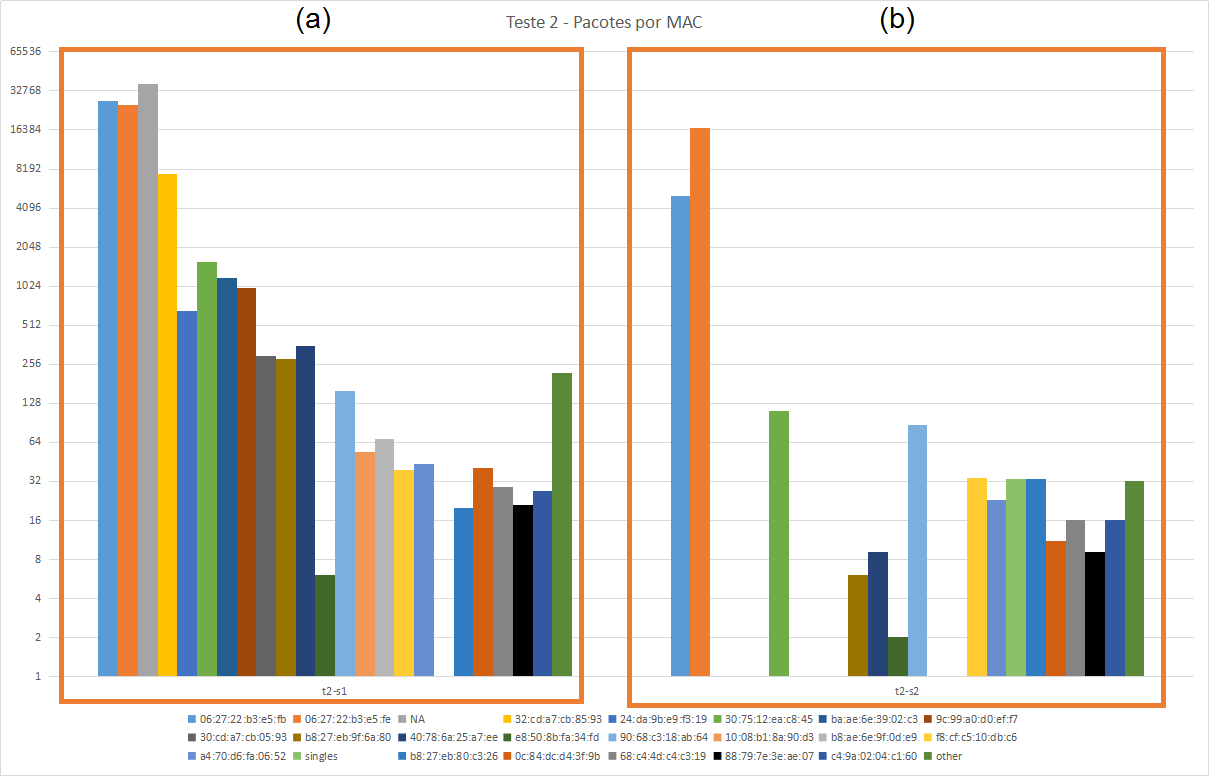
\includegraphics[width=1\textwidth]{060-testes/data-analisis/distance-mg4plus-netflix/Teste2.png}
		\legend{Fonte: Elaborada pelo autor}
	\end{minipage}
\end{figure}


\begin{figure}[htb]
	\label{mg4-distance}
	\centering
	\begin{minipage}{0.49\textwidth}
	\centering
		\caption{\label{fig-mg4-t1}dBm Motorola G4+ - Teste 1}
		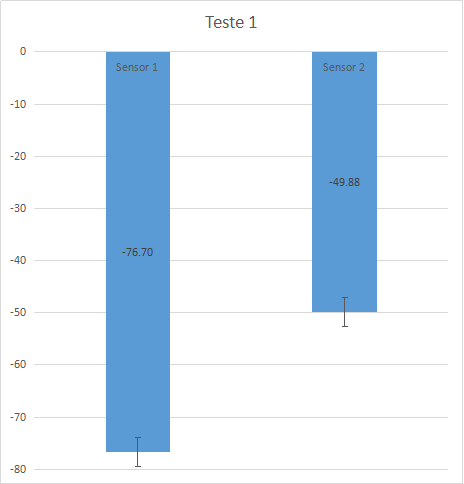
\includegraphics[width=1\textwidth]{060-testes/data-analisis/distance-mg4plus-netflix/target-Teste1.png}
		\legend{Fonte: Elaborada pelo autor}
	\end{minipage}
	\hfill
	\begin{minipage}{0.49\textwidth}
	\centering
		\caption{\label{fig-mg4-t2}dBm Motorola G4+ - Teste 2}
		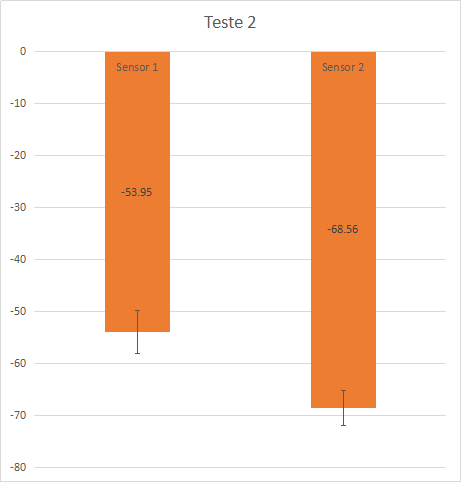
\includegraphics[width=1\textwidth]{060-testes/data-analisis/distance-mg4plus-netflix/target-Teste2.png}
		\legend{Fonte: Elaborada pelo autor}
	\end{minipage}
\end{figure}
